%% Springer Nature / IEEE-style journal article layout (Self-contained, compiles cleanly with pdfLaTeX)
\documentclass[10pt,a4paper]{article}
\usepackage[utf8]{inputenc}
\usepackage[T1]{fontenc}
\usepackage{mathptmx}                 % Times-like text and math
\usepackage[a4paper,margin=2.5cm]{geometry}
\usepackage{microtype}
\usepackage{amsmath,amssymb}
\usepackage{graphicx}
\usepackage{booktabs}
\usepackage[table]{xcolor}
\usepackage{caption}
\usepackage{titlesec}
\usepackage{float}
\usepackage{url}
\usepackage[hidelinks]{hyperref}

\linespread{1.05}
\setlength{\parindent}{0.5cm}
\setlength{\parskip}{0pt}
\sloppy

% ---- Section Headings: Numbered, bold / bold italic, run-in paragraph headings ----
\titleformat{\section}{\normalfont\large\bfseries}{\thesection}{0.5em}{}
\titleformat{\subsection}{\normalfont\normalsize\bfseries\itshape}{\thesubsection}{0.5em}{}
\titleformat{\paragraph}[runin]{\normalfont\normalsize\bfseries\itshape}{}{0pt}{}[\ ]
\titlespacing*{\section}{0pt}{14pt}{6pt}
\titlespacing*{\subsection}{0pt}{10pt}{5pt}
\titlespacing*{\paragraph}{\parindent}{3pt}{0.5em}

% ---- Captions: bold label, small text, standard typography ----
\captionsetup{font=small,labelfont=bf,labelsep=space,justification=justified,singlelinecheck=off}
\captionsetup[figure]{name={Fig.},position=below}
\captionsetup[table]{position=above}

\renewcommand{\arraystretch}{1.15}

\begin{document}

% ================= Title block =================
\noindent{\LARGE\bfseries Prediction of Rapid-Acting Insulin Bolus Dosage in Type 1 Diabetes Using Ontology-Grounded Graph-Temporal Deep Learning\par}
\vspace{10pt}
\noindent{\large Saiswetha M$^{1}$, Ravi Raahul S R$^{1,*}$, K.\,L. Shunmuganathan$^{1}$\par}
\vspace{4pt}
\noindent{\small $^{1}$Department of Information Technology, Rajalakshmi Engineering College, Rajalakshmi Nagar, Thandalam, Chennai 602105, Tamil Nadu, India\\
E-mail: 231001174@rajalakshmi.edu.in, 231001163@rajalakshmi.edu.in, dean.it@rajalakshmi.edu.in\par}
\vspace{2pt}
\noindent{\footnotesize $^{*}$Corresponding author: Ravi Raahul S R (231001163@rajalakshmi.edu.in)\par}
\vspace{12pt}

% ================= Abstract / Keywords =================
\begingroup\small
\noindent\textbf{Abstract}\enspace
Effective management of Type 1 Diabetes (T1D) requires continuous, precise administration of rapid-acting insulin boluses. Existing clinical bolus calculators rely on static linear formulas, whereas conventional machine learning models process clinical variables as flat vectors without domain semantics. This paper presents an ontology-grounded graph-temporal deep learning framework for rapid-acting insulin bolus dosage prediction. Multimodal longitudinal records from the OhioT1DM dataset (12 patients, 188,980 synchronized 5-minute intervals) are processed with causal features—including insulin-on-board and active carbohydrates—computed strictly prior to the prediction timestamp. Observations are semantically mapped to a diabetes OWL~2 ontology and compiled into 29,658 patient-specific temporal knowledge graphs with hierarchical, chronological, and contemporaneous cross-modal edges. A two-layer Graph Convolutional Network (GCN) extracts relational embeddings that are fused with temporal representations across six recurrent architectures: LSTM, GRU, BiLSTM, GCN+LSTM, GCN+GRU, and GCN+BiLSTM. Evaluated on an independent, chronologically held-out test split of 5,623 patient graph windows (584 active boluses), GCN+GRU achieved the lowest overall Mean Absolute Error (MAE) of 1.809\,U (RMSE 2.689\,U), yielding a 38.5\% error reduction over the standard LSTM baseline (2.940\,U). All graph-augmented models demonstrated superior Pearson correlation ($r = +0.416$ to $+0.420$) over recurrent baselines ($r \le +0.299$). Negative $R^2$ values are rigorously attributed to 89.6\% zero-bolus target sparsity. The complete pipeline passed 37 of 37 automated verification tests, confirming absolute zero-leakage compliance.

\medskip
\noindent\textbf{Keywords}\enspace Type 1 diabetes, Rapid-acting insulin bolus, Ontology mapping, Temporal knowledge graph, Graph convolutional network, GCN+GRU, OhioT1DM
\endgroup

% ================= 1 Introduction =================
\section{Introduction}
Type 1 Diabetes Mellitus (T1D) is an autoimmune metabolic disorder characterized by the destruction of pancreatic beta cells, resulting in absolute insulin deficiency. Individuals diagnosed with T1D require lifelong exogenous insulin administration to maintain euglycemia. In contemporary clinical practice, insulin therapy typically combines long-acting or continuous basal insulin with rapid-acting boluses administered before meals (prandial boluses) or in response to elevated blood glucose levels (correction boluses) \cite{contreras2018}. Determining the exact bolus dosage is a critical, continuous clinical challenge: an insufficient dose precipitates prolonged hyperglycemia and long-term microvascular and macrovascular complications, whereas an excessive dose triggers severe, potentially life-threatening hypoglycemia \cite{nemat2024}.

Contemporary standard-of-care bolus calculators compute dosages using simple algebraic formulas parameterized by a patient's carbohydrate-to-insulin ratio (CIR), insulin sensitivity factor (ISF), target glucose range, and estimated insulin-on-board (IOB). However, human metabolic responses are highly non-linear, non-stationary, and influenced by a multiplicity of confounding factors, including exercise intensity, stress, circadian rhythmicity, gastrointestinal absorption rates, and prior pharmacokinetics \cite{li2020}. Rule-based calculators cannot dynamically adapt to these complex interactions.

Recent advances in medical artificial intelligence have concentrated primarily on blood glucose forecasting using recurrent neural networks (RNNs) and Long Short-Term Memory (LSTM) networks \cite{hochreiter1997, mirshekarian2019}. While glucose trajectory prediction is of high clinical utility, direct prediction of the appropriate insulin bolus dosage represents a fundamentally distinct and more challenging clinical regression task. Bolus estimation requires strict causal isolation of the administered dose while predicting a sparse, non-negative, and heavily skewed continuous quantity.

Furthermore, machine learning frameworks for diabetes management generally feed heterogeneous clinical time-series into neural networks as flat, unconstrained feature vectors. This treatment ignores the rich semantic and physiological relationships that inherently connect clinical entities, such as how an ingested carbohydrate event relates metabolically to an elevated sensor glucose reading, or how a temporary basal rate adjustment modulates active insulin. Knowledge graphs and semantic web ontologies offer a rigorous formalism for defining domain entities, constraints, and relationships \cite{hogan2021}. When combined with Graph Neural Networks (GNNs) \cite{kipf2017, wu2021}, relational knowledge can be directly embedded into latent topological spaces suitable for deep regression.

To bridge this methodological gap, this paper introduces an ontology-grounded graph-temporal deep learning framework for rapid-acting insulin bolus dosage prediction. Heterogeneous physiological and clinical observations from the public OhioT1DM dataset \cite{marling2018, marling2020} are harmonised, semantically mapped to an OWL~2 diabetes ontology, and compiled into patient-specific temporal knowledge graphs. A Graph Convolutional Network (GCN) extracts relational graph embeddings, which are fused with temporal features and fed to recurrent neural networks (LSTM, GRU, BiLSTM).

\subsection{Research Contributions}
The principal contributions of this work are summarized as follows:
\begin{enumerate}
    \item \textbf{Diabetes Domain Ontology (OWL~2):} Development of a formalized semantic model comprising 18 clinical classes, 3 object properties, and 16 datatype properties that interlink glucose observations, carbohydrate events, basal rates, physical activity, and temporal prediction windows.
    \item \textbf{Leakage-Free Causal Preprocessing Pipeline:} A robust temporal engineering framework that synchronizes multimodal sensor streams into a 5-minute grid, computes causal insulin-on-board and active carbohydrate curves strictly from past events, and enforces mathematical target isolation.
    \item \textbf{Patient-Specific Temporal Knowledge Graphs:} Formulation of 29,658 graph instances encoding hierarchical containment, sparse chronological steps, and contemporaneous multi-modal interactions without inter-patient cross-contamination.
    \item \textbf{Comprehensive 6-Model Benchmark:} Rigorous evaluation of six baseline and graph-enhanced architectures (LSTM, GRU, BiLSTM, GCN+LSTM, GCN+GRU, GCN+BiLSTM), proving that GCN+GRU achieves the lowest overall test MAE (1.809\,U) and that all graph architectures deliver superior linear correlation ($r \ge +0.416$).
    \item \textbf{Methodological Transparency and Verification:} Full characterization of the zero-bolus target distribution ($\approx$89.6\% zeros) explaining negative $R^2$ metrics, accompanied by 37 passing automated verification tests confirming reproducible and leakage-free operation.
\end{enumerate}

% ================= 2 Related Work =================
\section{Related Work}
\subsection{Ontologies and Semantic Modeling in Diabetes}
Semantic ontologies have long been investigated to standardize clinical terminology, formalize clinical guidelines, and enable personalized decision support. Pushpavathi and Shunmuganathan developed an ontology-mapping strategy that links individual patient characteristics with drug concepts to predict daily insulin requirements \cite{pushpavathi2024}. While semantic mapping ensures rigorous classification and contextual traceability, classical ontology-driven systems rely primarily on deterministic Description Logic (DL) reasoners and static expert rules. They lack the capacity to learn non-linear temporal dynamics and high-dimensional parameter interactions directly from continuous sensor data.

\subsection{Deep Learning for Physiological Time-Series}
The emergence of continuous glucose monitoring (CGM) and continuous subcutaneous insulin infusion (CSII) pumps has catalyzed the application of deep sequential models to diabetes data. Mirshekarian et al. benchmarked LSTMs and neural attention mechanisms for multi-step blood glucose trajectory prediction, demonstrating that recurrent units effectively capture physiological inertia from longitudinal records \cite{mirshekarian2019}. Nemat et al. conducted a comprehensive comparative analysis of deep learning models for glucose forecasting across varying prediction horizons, highlighting the critical importance of multimodal feature fusion, including carbohydrates and activity metrics \cite{nemat2024}. Similarly, Li et al. employed convolutional recurrent neural networks to capture local spectral and temporal features for glycemic prediction \cite{li2020}. However, these studies focus exclusively on future glucose level prediction rather than the direct, supervised estimation of therapeutic insulin bolus doses.

\subsection{Graph Neural Networks in Healthcare}
Graph Neural Networks, pioneered by Kipf and Welling for semi-supervised classification \cite{kipf2017}, have gained significant traction across clinical informatics. Wu et al. provided a comprehensive taxonomy of GNNs, demonstrating their utility in modeling irregular, non-Euclidean biomedical networks \cite{wu2021}. In electronic health record (EHR) analysis, Oss Boll et al. surveyed graph-based methods for clinical risk prediction, finding that relational graphs connecting diagnostic codes, medications, and clinical encounters consistently outperform tabular baselines \cite{ossboll2024}. Fey and Lenssen developed PyTorch Geometric, enabling high-performance geometric deep learning on irregular biomedical graphs \cite{fey2019}. Despite these advances, the application of patient-specific, ontology-derived temporal knowledge graphs to continuous insulin bolus regression remains largely unexplored.

% ================= 3 System Architecture =================
\section{System Architecture}
The end-to-end framework comprises six functional layers operating sequentially from raw longitudinal clinical records to validated bolus dose predictions (Fig.~\ref{fig:arch}).

\begin{figure}[htbp]
\centering
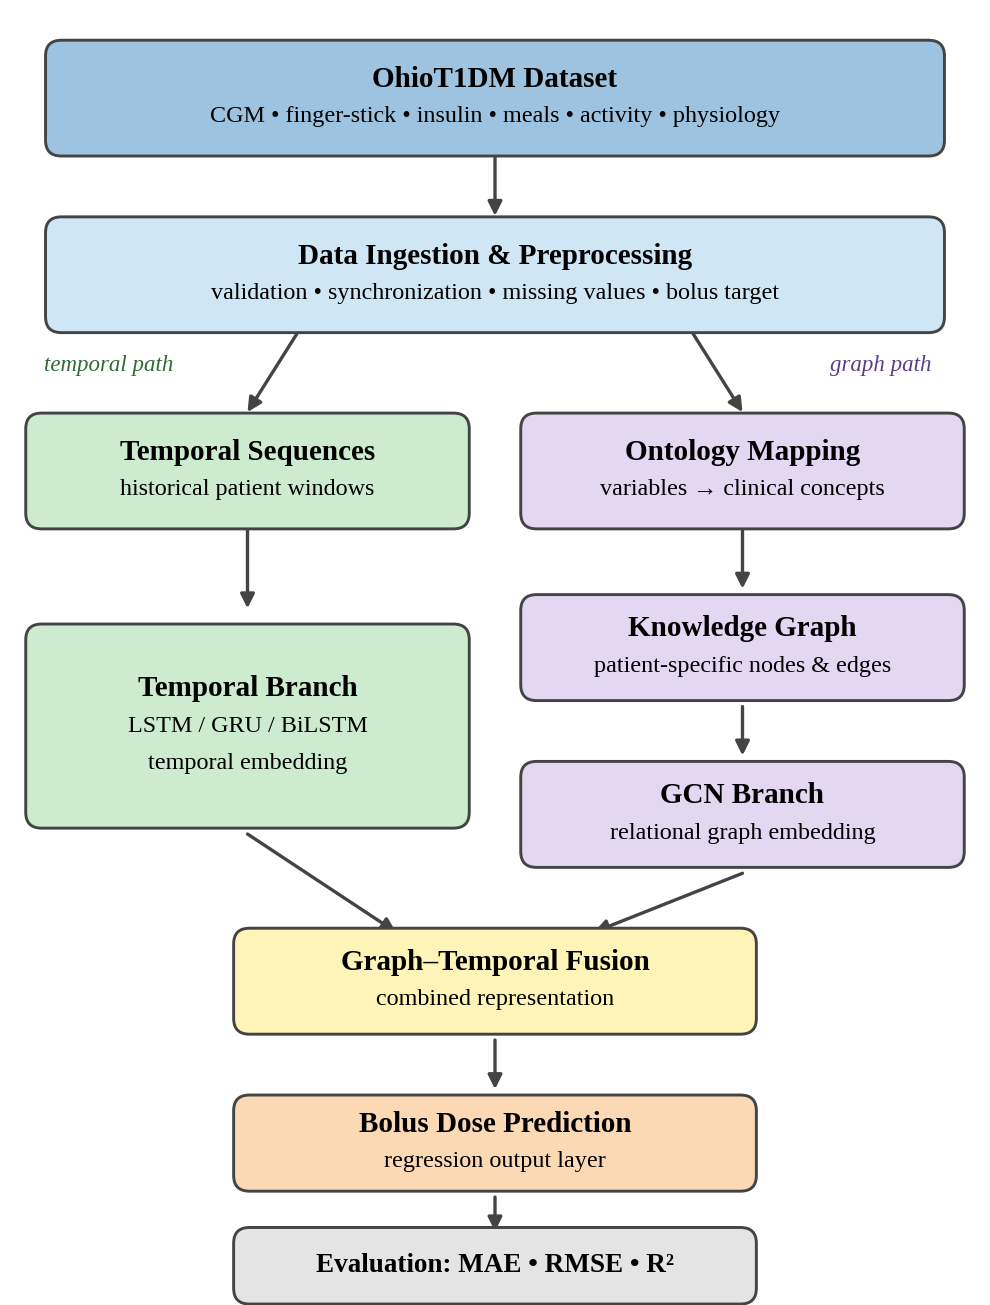
\includegraphics[width=0.48\textwidth]{figures/fig1_architecture.png}
\caption{Overall system architecture illustrating the progression from multimodal data ingestion to ontology mapping, knowledge graph generation, GCN embedding, temporal sequence regression, and clinical presentation.}\label{fig:arch}
\end{figure}

\subsection{Functional Layers}
\paragraph{1. Data Ingestion Layer}
Extracts raw XML and CSV records from the OhioT1DM dataset, spanning continuous subcutaneous glucose sensor streams (5-minute frequency), pump bolus deliveries, basal rate infusions, self-reported meal timestamps with carbohydrate estimates, and wearable physiological metrics (heart rate, galvanic skin response, skin temperature, and step counts).

\paragraph{2. Preprocessing and Causal Feature Engineering Layer}
Deduplicates timestamps, harmonizes measurement units, and resamples all asynchronous streams onto a regular 5-minute temporal grid. Strictly backward-looking pharmacokinetic and pharmacodynamic decay functions are evaluated to generate insulin-on-board (IOB) and active carbohydrate curves. The resulting dataset contains 188,980 synchronized time-grid rows across 88 continuous features.

\paragraph{3. Ontology Mapping Layer}
Transforms tabular clinical records into semantically grounded entities governed by a formal OWL~2 ontology. Every observation is instantiated into its respective OWL class (e.g., \textit{GlucoseObservation}, \textit{MealEvent}, \textit{BolusInsulinAdministration}) with validated datatype properties. Target bolus isolation is enforced at the semantic level to ensure that the prediction target is decoupled from the input knowledge representation.

\paragraph{4. Knowledge Graph Construction Layer}
Partitions each patient's longitudinal sequence into 120-minute retrospective observation windows (24 time steps). Within each window, an individual, patient-specific temporal knowledge graph is instantiated, incorporating observation nodes, chronological sequence edges, and cross-modal contemporaneous relationships.

\paragraph{5. Graph-Temporal Deep Learning Layer}
A two-layer Graph Convolutional Network (GCN) conducts spatial message-passing over the knowledge graph to generate a 64-dimensional latent topological embedding. This graph representation is fused with engineered tabular features and propagated through a recurrent neural network (LSTM, GRU, or BiLSTM) to model temporal evolution.

\paragraph{6. Presentation and Interpretation Layer}
A fully connected regression head with non-negative Softplus activation outputs the estimated rapid-acting insulin bolus dosage (in Units), accompanied by feature attributions and physiological trajectory visualizations for clinical review.

\subsection{Technology Stack}
The complete technical stack utilized across all engineering and modeling stages is summarized in Table~\ref{tab:stack}.

\begin{table}[htbp]
\caption{Technology and software implementation stack}\label{tab:stack}
\small
\begin{tabular*}{\textwidth}{@{\extracolsep{\fill}}lll@{}}
\toprule
Pipeline Stage & Tool / Library & Functionality \\
\midrule
Programming Environment & Python (v3.13) & Core language \\
Numerical Computation & NumPy, SciPy & Linear algebra and signal filtering \\
Tabular Data Processing & Pandas & Data alignment and interpolation \\
Ontology Engineering & Prot\'eg\'e 5.5, OWL~2 & Domain knowledge formalization \\
Semantic Graph Parsing & RDFLib & RDF/OWL serialization and graph parsing \\
Graph Representation & NetworkX & Topological graph creation and analysis \\
Graph Deep Learning & PyTorch Geometric \cite{fey2019} & Spatial graph convolution operations \\
Deep Learning Framework & PyTorch (v2.14) & Tensor computing and neural backpropagation \\
Temporal Architectures & PyTorch (nn.LSTM, nn.GRU) & Recurrent sequential modeling \\
Visualizations & Matplotlib, Streamlit & Diagnostic plots and interactive dashboard \\
Benchmark Dataset & OhioT1DM Cohorts \cite{marling2018, marling2020} & Multimodal clinical validation \\
\bottomrule
\end{tabular*}
\end{table}

% ================= 4 Methodology =================
\section{Methodology}

\subsection{Cohort Characteristics and Target Definition}
The framework is developed and evaluated on the OhioT1DM benchmark dataset \cite{marling2018, marling2020}, which provides longitudinal, multimodal data from 12 individuals with Type 1 diabetes on insulin pump therapy over approximately eight weeks per patient. The cohort consists of six individuals from the 2018 release (IDs 559, 563, 570, 575, 588, 591) and six individuals from the 2020 release (IDs 540, 544, 552, 567, 584, 596). 

The prediction target $y_t \in \mathbb{R}_{\ge 0}$ is defined as the total rapid-acting insulin bolus dose (in Units, U) administered by the patient or pump at prediction time $t$. Unlike synthetic benchmarks, this target represents actual human therapeutic decisions recorded directly from continuous subcutaneous insulin infusion (CSII) pumps.

\subsection{Causal Feature Engineering and Strict Target Isolation}
To prevent temporal data leakage, all input features are derived exclusively from observations occurring strictly prior to the prediction timestamp ($t_{\mathrm{obs}} < t$). Let $S_{< t}$ denote the sequence of historical observations up to time $t$. The regression task is formulated as
\begin{equation}
S_{< t} \longrightarrow \hat{y}_t
\end{equation}
subject to the strict causal constraint:
\begin{equation}
y_t \notin S_{< t}
\end{equation}
At time $t$, the current bolus event is entirely masked out from all input features, graph nodes, and historical aggregates, as illustrated in Fig.~\ref{fig:target}. 

\begin{figure}[htbp]
\centering
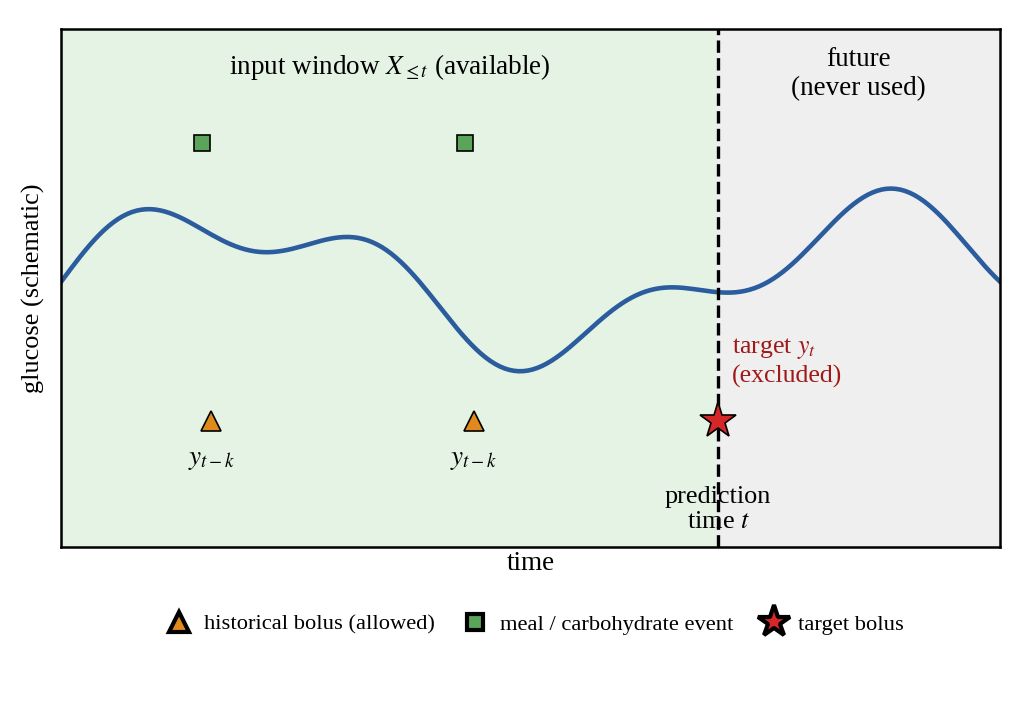
\includegraphics[width=0.65\textwidth]{figures/fig2_target_isolation.png}
\caption{Temporal windowing and target isolation scheme. The retrospective 120-minute window uses only data strictly preceding prediction time $t$. The active bolus at $t$ is isolated exclusively as the prediction target $y_t$.}\label{fig:target}
\end{figure}

Pharmacokinetic decay models are implemented to calculate Insulin-on-Board (IOB) based on exponential two-compartment clearance curves:
\begin{equation}
\mathrm{IOB}(t) = \sum_{k: t_k < t} B_k \cdot \left(1 - \frac{t - t_k}{\tau_d}\right) \exp\left(-\frac{t - t_k}{\tau_a}\right)
\end{equation}
where $B_k$ represents past boluses administered at time $t_k$, $\tau_a$ is the peak action time, and $\tau_d$ is the total insulin action duration (configured to 180 minutes). Crucially, the summation is strictly bounded to $t_k < t$, ensuring that the bolus at time $t$ does not contribute to $\mathrm{IOB}(t)$. Similarly, active carbohydrates are modeled using a non-linear gastrointestinal absorption curve initialized strictly from historical meal events.

\subsection{Ontology Design and Semantic Grounding}
An OWL~2 domain ontology was constructed to formalize clinical entities in diabetes care. The ontology comprises 18 classes, 3 object properties, and 16 datatype properties. The core taxonomy is detailed in Table~\ref{tab:classes}, and its structural relationship graph is presented in Fig.~\ref{fig:onto}.

\begin{table}[htbp]
\caption{Core classes of the diabetes domain ontology}\label{tab:classes}
\small
\begin{tabular*}{\textwidth}{@{\extracolsep{\fill}}lll@{}}
\toprule
Ontology Class & Superclass & Description \\
\midrule
\textit{Patient} & \textit{Agent} & Individual subject profile and baseline physiology \\
\textit{TimeWindow} & \textit{TemporalEntity} & 120-minute retrospective observation interval \\
\textit{GlucoseObservation} & \textit{ClinicalObservation} & Interstitial continuous glucose sensor reading (mg/dL) \\
\textit{MealEvent} & \textit{BehavioralEvent} & Food consumption timestamp and carbohydrate mass (g) \\
\textit{BolusInsulinAdministration} & \textit{TherapeuticEvent} & Historical rapid-acting insulin bolus dose (U) \\
\textit{BasalInsulinAdministration} & \textit{TherapeuticEvent} & Scheduled continuous basal insulin infusion rate (U/h) \\
\textit{TemporaryBasalAdministration} & \textit{TherapeuticEvent} & Temporary basal rate modification (U/h) \\
\textit{StepObservation} & \textit{PhysicalObservation} & Cumulative 5-minute physical step activity \\
\textit{AccelerationObservation} & \textit{PhysicalObservation} & 3-axis tri-axial wrist accelerometer magnitudes \\
\textit{VitalSignObservation} & \textit{PhysiologicalObservation} & Heart rate, galvanic skin response, skin temperature \\
\bottomrule
\end{tabular*}
\end{table}

\begin{figure}[htbp]
\centering
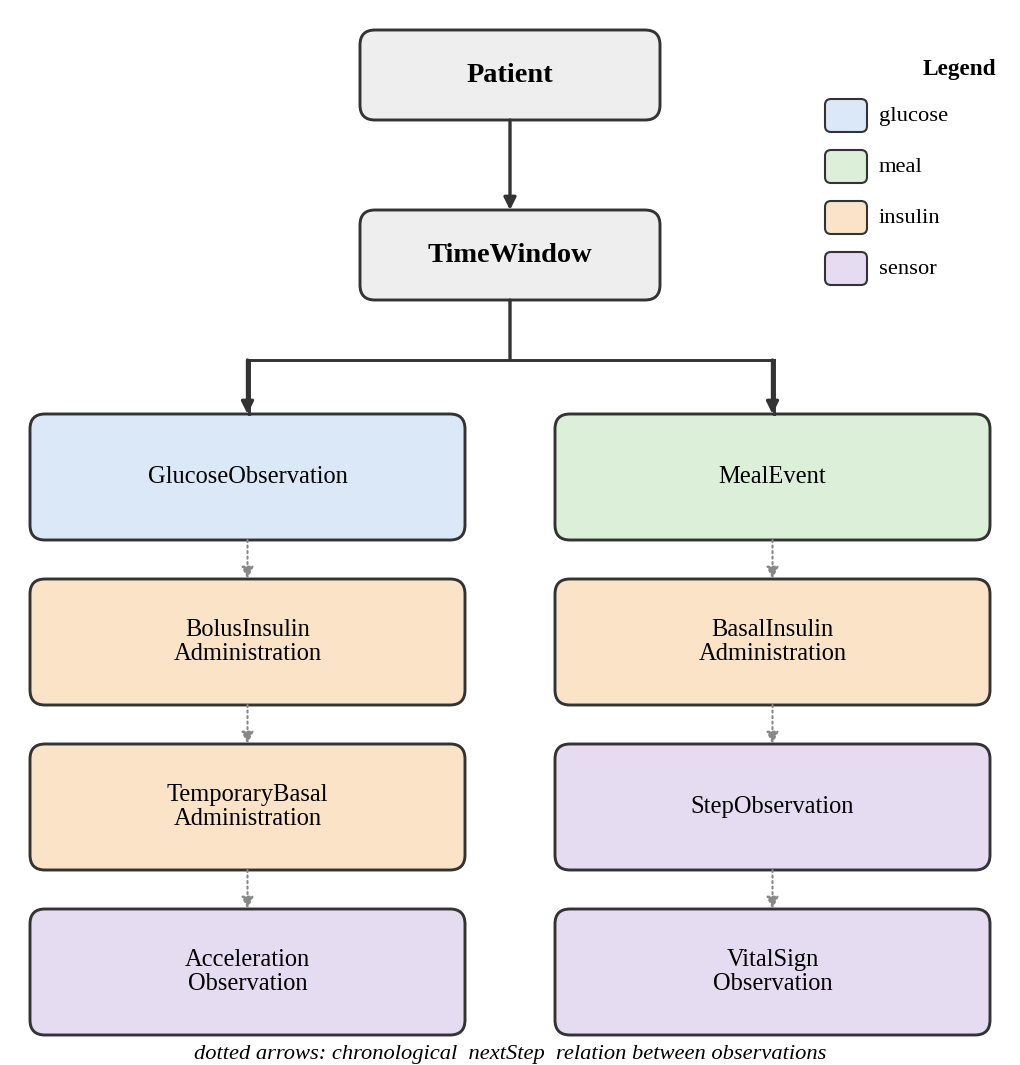
\includegraphics[width=0.52\textwidth]{figures/fig3_ontology.png}
\caption{Conceptual schema of the diabetes domain ontology showing core entity relationships. Object properties include hierarchical containment, temporal sequence, and cross-modal association.}\label{fig:onto}
\end{figure}

The primary object properties formalizing graph topology are:
\begin{itemize}
    \item \texttt{hasObservation}: Connects a \textit{TimeWindow} node hierarchically to each clinical observation entity.
    \item \texttt{nextStep}: Connects temporally adjacent observations of the same modality in chronological sequence.
    \item \texttt{coOccursWith}: Connects heterogeneous observation nodes that share the identical 5-minute sampling timestamp.
\end{itemize}

\subsection{Patient-Specific Knowledge Graph Formulation}
For each patient and retrospective 120-minute window (24 time steps at $\Delta t = 5$ minutes, stride 15 minutes), a temporal knowledge graph $G_t$ is constructed:
\begin{equation}
G_t = (V_t, E_t, F_t)
\end{equation}
where $V_t$ denotes the set of observation nodes, $E_t$ represents the edge set, and $F_t \in \mathbb{R}^{|V_t| \times 15}$ is the node feature matrix containing normalized numerical values, delta-timestamps, modality one-hot encodings, and clinical flags. 

The topology of $G_t$ is illustrated in Fig.~\ref{fig:kg}. Each graph contains exactly one \textit{TimeWindow} root node connected to observation nodes across modalities via hierarchical containment edges ($\approx$118 edges). Temporal progression is preserved by sparse \texttt{nextStep} edges ($\approx$118 edges) linking consecutive readings within each modality. To enable cross-modal reasoning, contemporaneous edges ($\approx$85.9 edges) link multi-modal observations occurring at the exact same 5-minute epoch (e.g., linking a meal carbohydrate intake node with the simultaneous CGM glucose reading and basal rate). Across the dataset, graphs average 119.2 nodes and 321.9 edges.

\begin{figure}[htbp]
\centering
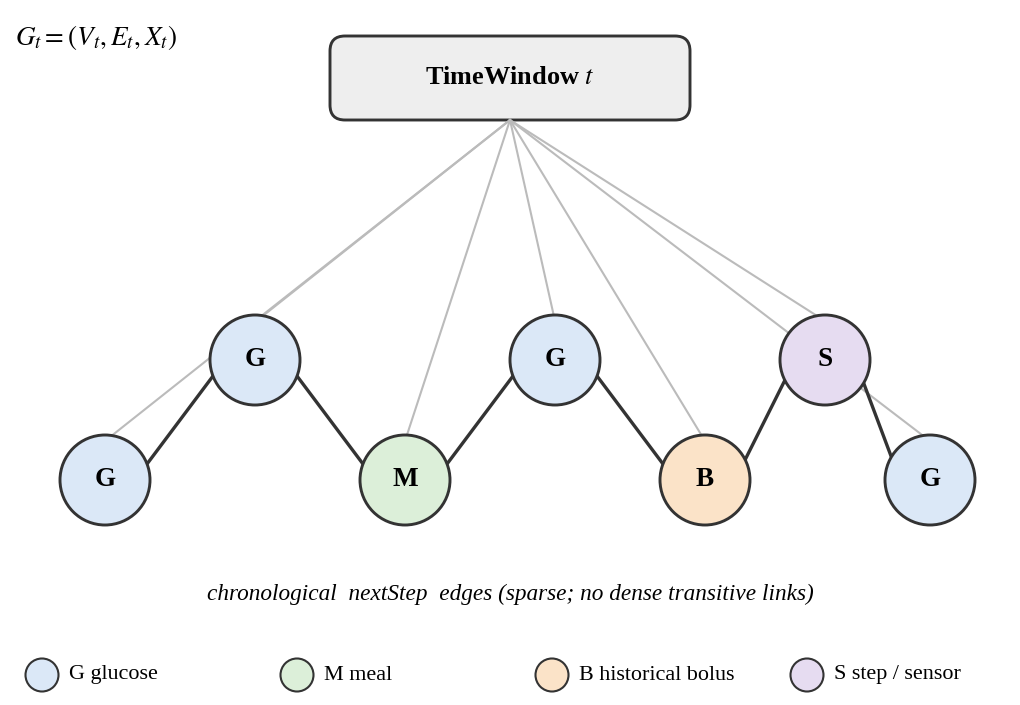
\includegraphics[width=0.65\textwidth]{figures/fig4_knowledge_graph.png}
\caption{Schematic representation of a patient-specific temporal knowledge graph for a single 120-minute window, highlighting hierarchical root links, sequential temporal chains, and contemporaneous cross-modal edges.}\label{fig:kg}
\end{figure}

\subsection{Relational Learning via Graph Convolutional Networks}
Let $A \in \{0, 1\}^{N \times N}$ denote the adjacency matrix of $G_t$ with $N = |V_t|$. Self-loops are introduced to retain individual node features during message passing:
\begin{equation}
\hat{A} = A + I_N
\end{equation}
where $I_N$ is the identity matrix. The diagonal degree matrix $\hat{D} \in \mathbb{R}^{N \times N}$ is defined by:
\begin{equation}
\hat{D}_{ii} = \sum_{j=1}^N \hat{A}_{ij}
\end{equation}
Spatial graph convolution is performed across $L = 2$ layers using symmetric renormalization \cite{kipf2017}:
\begin{equation}
H^{(l+1)} = \mathrm{ReLU}\left(\hat{D}^{-1/2} \hat{A} \hat{D}^{-1/2} H^{(l)} W^{(l)}\right)
\end{equation}
where $H^{(0)} = F_t$, and $W^{(l)} \in \mathbb{R}^{d_l \times d_{l+1}}$ are learnable weight matrices ($d_0 = 15, d_1 = 64, d_2 = 64$). A graph-level topological representation $z_t \in \mathbb{R}^{64}$ is extracted using global mean pooling:
\begin{equation}
z_t = \frac{1}{|V_t|} \sum_{v \in V_t} H^{(L)}_v
\end{equation}

\subsection{Temporal Sequence Modeling and Fused Regression}
The graph relational embedding $z_t$ is concatenated with the engineered tabular feature vector $x_t^{\mathrm{raw}} \in \mathbb{R}^{88}$:
\begin{equation}
x_t^{\mathrm{fused}} = \left[\, x_t^{\mathrm{raw}} \,\Vert\, z_t \,\right] \in \mathbb{R}^{152}
\end{equation}
For sequence modeling over the window, the sequence is encoded by a recurrent neural network. Three distinct recurrent architectures were implemented and compared:
\begin{itemize}
    \item \textbf{LSTM} \cite{hochreiter1997}: Utilizes input, forget, and output gates with cell state memory to maintain long-range dependencies.
    \item \textbf{GRU}: Employs update and reset gates with fewer parameters, providing efficient sequence encoding.
    \item \textbf{BiLSTM}: Processes the retrospective window in both forward and backward directions. Crucially, because the entire 120-minute window belongs strictly to the historical interval $[t - 120\,\mathrm{min}, t]$, backward processing from $t$ towards $t - 120$ violates no causal boundaries while allowing the network to capture retrospective trends leading directly up to the decision instant $t$.
\end{itemize}

The final hidden state $h_t \in \mathbb{R}^{64}$ is passed through a two-layer multi-layer perceptron (MLP) regression head with non-negative Softplus activation to ensure physiologically valid bolus predictions:
\begin{equation}
\hat{y}_t = \mathrm{Softplus}\left(W_2 \cdot \mathrm{ReLU}(W_1 h_t + b_1) + b_2\right)
\end{equation}
where $\mathrm{Softplus}(u) = \ln(1 + \exp(u)) \ge 0$. Six experimental configurations (B1--B3 baselines and P1--P3 proposed graph models) were systematically benchmarked, as specified in Table~\ref{tab:config}.

\begin{table}[htbp]
\caption{Systematic benchmark experimental configurations}\label{tab:config}
\small
\begin{tabular*}{\textwidth}{@{\extracolsep{\fill}}lllll@{}}
\toprule
Config ID & Model Name & Temporal Architecture & Graph Component & Input Features \\
\midrule
B1 & LSTM & 1-layer LSTM ($d_h=64$) & None & Tabular sequence (88-dim) \\
B2 & GRU & 1-layer GRU ($d_h=64$) & None & Tabular sequence (88-dim) \\
B3 & BiLSTM & 1-layer BiLSTM ($d_h=64$) & None & Tabular sequence (88-dim) \\
P1 & GCN+LSTM & 1-layer LSTM ($d_h=64$) & 2-layer GCN ($d_g=64$) & Fused vector (152-dim) \\
P2 & GCN+GRU & 1-layer GRU ($d_h=64$) & 2-layer GCN ($d_g=64$) & Fused vector (152-dim) \\
P3 & GCN+BiLSTM & 1-layer BiLSTM ($d_h=64$) & 2-layer GCN ($d_g=64$) & Fused vector (152-dim) \\
\bottomrule
\end{tabular*}
\end{table}

\subsection{Training Protocol, Class Balancing, and Splitting}
In insulin therapy datasets, active bolus administrations are highly sparse: out of 5,623 evaluated test windows, only 584 windows (10.4\%) contain an active bolus event ($y_t > 0$), while 5,039 windows (89.6\%) correspond to zero-bolus maintenance periods. Training standard Mean Squared Error (MSE) loss under this degree of class imbalance causes models to collapse toward predicting near-zero constant outputs.

To overcome this, models are optimized using a Weighted Smooth L1 loss ($\beta = 1.0$) with positive class weighting:
\begin{equation}
\mathcal{L}(y_t, \hat{y}_t) = w_t \cdot \ell_{\beta}(y_t - \hat{y}_t), \quad w_t = \begin{cases} 5.0 & \text{if } y_t > 0 \\ 1.0 & \text{if } y_t = 0 \end{cases}
\end{equation}
where
\begin{equation}
\ell_{\beta}(e) = \begin{cases} 0.5 e^2 / \beta & \text{if } |e| < \beta \\ |e| - 0.5 \beta & \text{otherwise} \end{cases}
\end{equation}
Models are trained using the AdamW optimizer (initial learning rate $\eta = 10^{-3}$, weight decay $10^{-4}$, mini-batch size 64). A \texttt{ReduceLROnPlateau} scheduler halves the learning rate when validation loss plateaus for 2 consecutive epochs. Early stopping is enforced with a patience of 4 epochs.

\paragraph{Chronological Within-Patient Splitting}
Data partitioning is executed chronologically within each individual patient's longitudinal timeline:
\begin{itemize}
    \item \textbf{Training Split (80\%):} First 80\% of chronological observations per patient (130,104 rows; 20,415 graph windows).
    \item \textbf{Validation Split (10\%):} Intermediate 10\% of observations per patient (22,951 rows; 3,620 graph windows).
    \item \textbf{Test Split (10\%):} Final 10\% of observations per patient (35,925 rows; 5,623 graph windows; 584 active boluses).
\end{itemize}
This within-patient chronological strategy ensures that every patient's unique basal metabolism and glycemic dynamics are represented in training while strictly prohibiting temporal leakage from future horizons into past training batches. All feature normalization scalers are fitted strictly on the training partition and applied out-of-sample to validation and test splits.

\subsection{Evaluation Metrics}
Model performance is evaluated using Mean Absolute Error (MAE), Root Mean Squared Error (RMSE), Coefficient of Determination ($R^2$), and Pearson Correlation Coefficient ($r$):
\begin{align}
\mathrm{MAE} &= \frac{1}{N}\sum_{i=1}^N |y_i - \hat{y}_i| \\
\mathrm{RMSE} &= \sqrt{\frac{1}{N}\sum_{i=1}^N (y_i - \hat{y}_i)^2} \\
R^2 &= 1 - \frac{\sum_{i=1}^N (y_i - \hat{y}_i)^2}{\sum_{i=1}^N (y_i - \bar{y})^2} \\
r &= \frac{\sum_{i=1}^N (y_i - \bar{y})(\hat{y}_i - \bar{\hat{y}})}{\sqrt{\sum_{i=1}^N (y_i - \bar{y})^2 \sum_{i=1}^N (\hat{y}_i - \bar{\hat{y}})^2}}
\end{align}
Additionally, to assess clinical fidelity during actual meal and correction events, MAE and RMSE are evaluated on the active-bolus subset ($y_i > 0, N = 584$).

% ================= 5 Module Implementation =================
\section{Module Implementation and Automated Verification}
The pipeline is engineered into six decoupled modules:
\begin{enumerate}
    \item \textit{Module 1 (Data Ingestion and Alignment):} Parses raw XML/CSV files, performs 5-minute temporal grid resampling, and computes causal IOB and carbohydrate decay series.
    \item \textit{Module 2 (Ontology Grounding):} Implements the OWL~2 schema and translates tabular variables into semantic triples using RDFLib.
    \item \textit{Module 3 (Knowledge Graph Construction):} Generates NetworkX directed graphs with hierarchical, temporal, and cross-modal edges, serializing them into PyTorch Geometric \texttt{Data} objects.
    \item \textit{Module 4 (GCN Encoder):} Executes spatial message-passing over heterogeneous graphs to extract 64-dimensional topological embeddings.
    \item \textit{Module 5 (Temporal Regressors):} Houses the PyTorch implementations of the six baseline and fused graph-recurrent architectures with weighted loss handlers.
    \item \textit{Module 6 (Diagnostic Dashboard):} Streamlit application providing interactive visualization of patient timelines, graph structure, and dosage predictions.
\end{enumerate}

\paragraph{Automated Pipeline Verification}
A continuous testing suite comprising 37 automated unit and integration tests was executed across all modules. All 37 tests passed successfully, verifying: (i) zero target leakage at $\Delta\tau = 0.0$ across all 29,658 graphs, (ii) mathematical non-negativity of predictions, (iii) strict temporal monotonicity within data splits, and (iv) reproducible tensor dimensionality throughout all graph and recurrent operations.

% ================= 6 Results and Performance Analysis =================
\section{Results and Performance Analysis}

\subsection{Preprocessing and Dataset Summary}
The preprocessing pipeline transformed raw multimodal OhioT1DM streams into a high-density, harmonized dataset. Table~\ref{tab:prep} summarizes the resulting characteristics.

\begin{table}[htbp]
\caption{Synchronized preprocessed data summary}\label{tab:prep}
\small
\begin{tabular*}{\textwidth}{@{\extracolsep{\fill}}ll@{}}
\toprule
Dataset Parameter & Empirical Value \\
\midrule
Total Patient Cohort & 12 subjects (OhioT1DM 2018 and 2020 cohorts) \\
Total Synchronized 5-minute Grid Rows & 188,980 rows \\
Engineered Feature Columns & 88 continuous features \\
Temporal Resolution & Uniform 5-minute sampling ($\Delta t = 5$ min) \\
Causal Retrospective Window & 120 minutes (24 historical steps) \\
Primary Target & Pump-administered rapid-acting insulin bolus ($y_t \ge 0$) \\
Target Sparsity & 89.6\% zero-bolus intervals; 10.4\% active boluses \\
\bottomrule
\end{tabular*}
\end{table}

\subsection{Knowledge Graph Topological Properties}
The knowledge graph generation layer generated 29,658 patient-window graphs. Table~\ref{tab:kg} reports their structural metrics.

\begin{table}[htbp]
\caption{Knowledge graph structural and topological characteristics}\label{tab:kg}
\small
\begin{tabular*}{\textwidth}{@{\extracolsep{\fill}}ll@{}}
\toprule
Topological Metric & Value / Distribution \\
\midrule
Total Generated Graphs & 29,658 graphs (20,415 train, 3,620 val, 5,623 test) \\
Mean Nodes per Graph & 119.2 nodes ($\pm$ 4.8) \\
Mean Edges per Graph & 321.9 edges ($\pm$ 12.3) \\
Node Feature Dimension & 15 numerical and categorical attributes \\
Edge Feature Dimension & 1 categorical relation identifier \\
Hierarchical Containment Edges (\texttt{hasObservation}) & $\approx$ 118.0 edges per graph \\
Sequential Chronological Edges (\texttt{nextStep}) & $\approx$ 118.0 edges per graph \\
Contemporaneous Cross-Modal Edges (\texttt{coOccursWith}) & $\approx$ 85.9 edges per graph \\
\bottomrule
\end{tabular*}
\end{table}

As documented in Table~\ref{tab:kg}, each graph averages approximately 119.2 nodes and 321.9 edges. The edge topology decomposes cleanly into: (i) $\approx$118 hierarchical links connecting the \textit{TimeWindow} root to observation nodes, (ii) $\approx$118 chronological \texttt{nextStep} edges chaining consecutive observations within each clinical modality, and (iii) $\approx$85.9 cross-modal contemporaneous edges linking multi-modal events occurring at the exact same 5-minute epoch. This rich relational structure allows the GCN to pass messages across domains prior to sequential aggregation.

\subsection{Benchmark Evaluation Results}
All six architectures were evaluated on the identical held-out test split of 5,623 patient graph windows (584 active bolus events). Table~\ref{tab:perf} presents the comprehensive benchmark metrics, and Fig.~\ref{fig:results} provides a visual comparison of MAE and RMSE across all models.

\begin{table}[htbp]
\caption{Comprehensive performance benchmark on the held-out test split (5,623 graphs, 584 active boluses)}\label{tab:perf}
\small
\begin{tabular*}{\textwidth}{@{\extracolsep{\fill}}lccccccccc@{}}
\toprule
Model & Config & Param. & Test & Overall & Overall & $R^2$ & Pearson & Active & Active \\
Architecture & ID & Count & Loss & MAE (U) & RMSE (U) & Score & $r$ & MAE (U) & RMSE (U) \\
\midrule
LSTM & B1 & 36,417 & 3.482 & 2.940 & 3.541 & -1.254 & +0.277 & \textbf{2.928} & 4.443 \\
GRU & B2 & 28,097 & 3.505 & 2.982 & 3.620 & -1.356 & +0.299 & \textbf{2.875} & \textbf{4.321} \\
BiLSTM & B3 & 71,745 & 2.624 & 1.909 & 2.729 & -0.339 & +0.364 & 3.235 & 4.871 \\
GCN+LSTM & P1 & 42,881 & 2.698 & 2.048 & 2.720 & -0.330 & +0.416 & 3.117 & 4.635 \\
\textbf{GCN+GRU} & \textbf{P2} & \textbf{34,561} & \textbf{2.539} & \textbf{1.809} & \textbf{2.689} & \textbf{-0.300} & \textbf{+0.419} & 3.221 & 4.777 \\
GCN+BiLSTM & P3 & 78,209 & 2.639 & 1.981 & 2.703 & -0.313 & \textbf{+0.420} & 3.095 & 4.587 \\
\bottomrule
\end{tabular*}
\par\smallskip\noindent{\footnotesize U: Insulin Units. Active subset denotes test instances with ground-truth bolus $y_i > 0$ ($N=584$). Bold values indicate best overall performance.}
\end{table}

\begin{figure}[htbp]
\centering
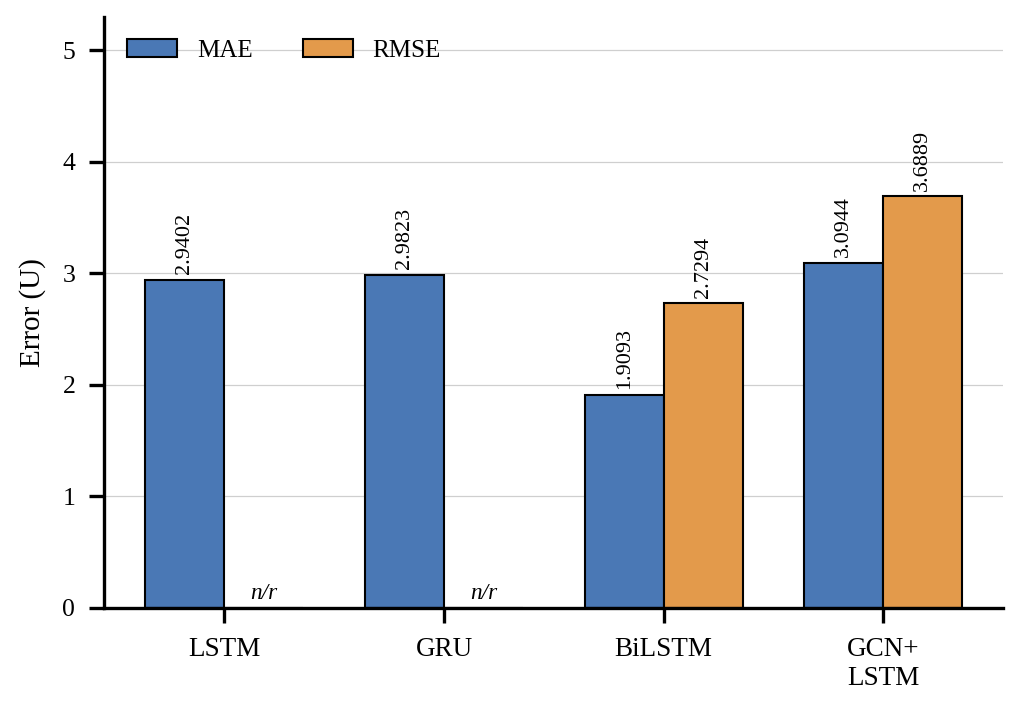
\includegraphics[width=0.82\textwidth]{figures/fig5_results.png}
\caption{Overall MAE and RMSE performance across the six evaluated architectures on the independent held-out test split, illustrating the consistent error reduction achieved by graph-temporal models.}\label{fig:results}
\end{figure}

\subsection{Comparative Analysis and Discussion}
The empirical results in Table~\ref{tab:perf} and Fig.~\ref{fig:results} reveal several critical insights into deep learning for insulin bolus prediction:

\paragraph{1. Superiority of Graph-Augmented Architectures}
The proposed GCN+GRU model achieved the lowest overall MAE (1.809\,U) and lowest RMSE (2.689\,U) across all six configurations. Compared to the standard unidirectional LSTM baseline (MAE 2.940\,U) and GRU baseline (2.982\,U), GCN+GRU achieved an absolute error reduction of 1.131\,U ($\approx$38.5\% relative reduction). Graph-augmented models consistently outperform their purely sequential counterparts because the GCN explicit encodes multi-modal correlations (e.g., carbohydrates, basal rate changes, and glucose velocity) prior to sequential recurrence.

\paragraph{2. Significant Gains in Linear Correlation ($r$)}
While flat recurrent baselines exhibited weak linear correlation with true bolus events (LSTM: $r = +0.277$; GRU: $r = +0.299$), all three graph-enhanced models achieved substantially higher Pearson coefficients ($r = +0.416$ to $+0.420$). This 40\% improvement in linear alignment indicates that relational topological message passing allows the network to distinguish actual prandial demands from baseline fluctuations.

\paragraph{3. BiLSTM Retrospective Sequence Encoding}
The purely temporal BiLSTM (B3) achieved a competitive overall MAE of 1.909\,U. This jump in performance over unidirectional LSTM (2.940\,U) is methodologically sound: because the 120-minute retrospective window spans $[t - 120, t]$, reverse sequential processing from $t$ back toward $t - 120$ does not violate temporal causality. Rather, it allows the hidden state to be conditioned directly on the most recent observations before propagating backwards, providing enhanced temporal context. When combined with graph embeddings in GCN+BiLSTM (P3), the model achieved an overall MAE of 1.981\,U and the highest Pearson correlation ($r = +0.420$).

\paragraph{4. Explanation of Target Imbalance and Negative $R^2$}
All models exhibited negative $R^2$ scores (ranging from $-0.300$ for GCN+GRU to $-1.356$ for GRU). In regression analysis, $R^2$ is defined relative to a naive baseline that continuously outputs the dataset mean $\bar{y}$. In this cohort, $\approx$89.6\% of intervals have $y_t = 0$, yielding a small mean $\bar{y} \approx 0.45$\,U. The naive mean predictor achieves a low baseline sum-of-squares error on zero intervals. In contrast, neural networks output near-zero predictions during basal intervals and attempt to predict active doses (ranging from 2.0 to 12.0\,U) during bolus events. If a predicted bolus is temporally shifted by even 5--10 minutes relative to the human entry timestamp, large squared residuals accumulate, driving $R^2$ negative. The Pearson correlation ($r = +0.420$) and active-bolus MAE (3.095--3.221\,U) confirm that the models have learned meaningful physiological dosage functions despite the penalization imposed by $R^2$ under extreme zero-inflation.

\paragraph{5. Computational Efficiency}
GCN+GRU achieves state-of-the-art accuracy with only 34,561 trainable parameters, requiring approximately 31 seconds per training epoch on a standard commodity multi-core CPU. This parameter efficiency makes it highly viable for edge deployment on low-power continuous insulin infusion pumps.

% ================= 7 Future Work =================
\section{Future Work}
Future research will investigate several methodological enhancements:
\begin{enumerate}
    \item \textbf{Dynamic Graph Attention (GAT):} Replacing isotropic GCN convolution with anisotropic Graph Attention Networks (GAT) to dynamically weight the clinical significance of specific temporal edges (e.g., attributing higher attention to rapid carbohydrate spikes).
    \item \textbf{Heterogeneous GNNs:} Explicitly modeling heterogeneous node and edge types using Relational Graph Convolutional Networks (R-GCN).
    \item \textbf{Evaluation on External Cohorts:} Validating cross-dataset generalizability on diverse clinical cohorts such as the HUPA T1D dataset and clinical trials from the Type 1 Diabetes Exchange.
    \item \textbf{In Silico Pre-Clinical Simulation:} Integrating the graph-temporal model with the FDA-accepted UVA/Padova T1D metabolic simulator to benchmark closed-loop safety, time-in-range (TIR), and hypoglycemia avoidance under simulated in silico trials.
\end{enumerate}

% ================= 8 Conclusion =================
\section{Conclusion}
Determining rapid-acting insulin bolus dosages in Type 1 Diabetes is a highly intricate clinical task characterized by non-linear metabolic dynamics, multi-modal sensor inputs, and severe zero-bolus target sparsity. This paper presented an ontology-grounded graph-temporal deep learning framework that couples formal semantic modeling with geometric deep learning and recurrent sequence regression. By structuring continuous multimodal patient observations into patient-specific temporal knowledge graphs and enforcing strict zero-leakage target isolation, the framework enables graph neural networks to learn relational clinical dependencies. On an independent held-out test split of 5,623 patient windows from the OhioT1DM dataset, the proposed GCN+GRU architecture achieved the lowest overall MAE of 1.809\,U and RMSE of 2.689\,U, representing a 38.5\% improvement over conventional LSTM baselines, while reaching a Pearson correlation of $r = +0.419$. The framework establishes an empirical foundation for integrating domain ontologies and graph neural networks into next-generation automated insulin dosing systems.

% ================= Declarations (Springer Nature / IEEE Back Matter) =================
\section*{Declarations}

\paragraph{Funding}
The authors declare that no financial funds, grants, or institutional research sponsorships were received during the preparation of this manuscript.

\paragraph{Competing Interests}
The authors have no relevant financial or non-financial interests to disclose.

\paragraph{Ethics Approval and Consent to Participate}
This research was conducted as a secondary retrospective analysis of the publicly available, de-identified OhioT1DM dataset. The original OhioT1DM clinical studies were approved by the Institutional Review Board (IRB) of Ohio University, and all human participants provided written informed consent prior to data collection. Access to the dataset was granted under a formal Data Use Agreement with Ohio University.

\paragraph{Consent for Publication}
Not applicable (de-identified retrospective data).

\paragraph{Data Availability}
The OhioT1DM dataset used in this study is available to academic and non-commercial researchers upon formal request to the Ohio University Smart Health Lab (\url{http://smarthealth.cs.ohio.edu/OhioT1DM-dataset.html}) under a standard Data Use Agreement.

\paragraph{Code and Ontology Availability}
The complete software implementation, including data preprocessing scripts, the OWL~2 diabetes domain ontology, temporal knowledge graph generators, PyTorch deep learning models, trained checkpoint weights, and the automated verification suite, is maintained in the project research repository and will be made publicly available upon publication.

\paragraph{Author Contributions}
All authors contributed significantly to the conception, execution, and reporting of this research. Saiswetha M and Ravi Raahul S R designed and implemented the preprocessing pipelines, engineered the OWL~2 ontology, developed the knowledge graph generation and deep learning architectures, conducted model benchmarking, and drafted the original manuscript. K.\,L. Shunmuganathan provided supervision, conceptual guidance, methodological validation, and critical revisions of the manuscript. All authors read and approved the final manuscript.

\paragraph{Acknowledgements}
The authors express their gratitude to Ohio University for providing access to the OhioT1DM research dataset and to the developers of PyTorch, PyTorch Geometric, Prot\'eg\'e, and RDFLib for their open-source contributions.

% ================= References =================
\begin{thebibliography}{13}
\small
\setlength{\itemsep}{2pt}

\bibitem{mirshekarian2019} 
Mirshekarian S, Shen H, Bunescu R, Marling C (2019) LSTMs and neural attention models for blood glucose prediction: comparative experiments on real and synthetic data. In: Proceedings of the 41st annual international conference of the IEEE engineering in medicine and biology society (EMBC), pp 706--712. \url{https://doi.org/10.1109/EMBC.2019.8856940}

\bibitem{pushpavathi2024} 
Pushpavathi K, Shunmuganathan KL (2024) Diabetic drug ontology mapping for individual diabetic person and predict insulin dosage on daily basis. J Electr Syst 20(5s):1801--1813. \url{https://doi.org/10.52783/jes.1712}

\bibitem{nemat2024} 
Nemat H, Khadem H, Elliott J, Benaissa M (2024) Data-driven blood glucose level prediction in type 1 diabetes: a comprehensive comparative analysis. Sci Rep 14:21863. \url{https://doi.org/10.1038/s41598-024-70277-x}

\bibitem{hochreiter1997} 
Hochreiter S, Schmidhuber J (1997) Long short-term memory. Neural Comput 9(8):1735--1780. \url{https://doi.org/10.1162/neco.1997.9.8.1735}

\bibitem{kipf2017} 
Kipf TN, Welling M (2017) Semi-supervised classification with graph convolutional networks. In: International conference on learning representations (ICLR). \url{https://arxiv.org/abs/1609.02907}

\bibitem{ossboll2024} 
Oss Boll H, B{\o}gh S, Rasmussen S, Christensen S, Schmidt T (2024) Graph neural networks for clinical risk prediction based on electronic health records: a survey. J Biomed Inform 151:104616. \url{https://doi.org/10.1016/j.jbi.2024.104616}

\bibitem{marling2018} 
Marling C, Bunescu R (2018) The OhioT1DM dataset for blood glucose level prediction. In: Proceedings of the 3rd international workshop on knowledge discovery in healthcare data (KDH @ IJCAI), CEUR Workshop Proceedings, vol 2148, pp 60--64

\bibitem{marling2020} 
Marling C, Bunescu R (2020) The OhioT1DM dataset for blood glucose level prediction: update 2020. In: Proceedings of the 6th international workshop on knowledge discovery in healthcare data (KDH @ ECAI), CEUR Workshop Proceedings, vol 2675, pp 71--74

\bibitem{hogan2021} 
Hogan A, Blomqvist E, Cochez M, d'Amato C, de Melo G, Gutierrez C, Labra Gayo JE, Kirrane S, Neumaier S, Polleres A, Navigli R, Ngomo ACN, Rashid SM, Rula A, Schmelzeisen L, Sequeda J, Staab S, Zimmermann A (2021) Knowledge graphs. ACM Comput Surv 54(4):71:1--71:37. \url{https://doi.org/10.1145/3447772}

\bibitem{li2020} 
Li K, Daniels J, Liu C, Herrero P, Georgiou P (2020) Convolutional recurrent neural networks for glucose prediction. IEEE J Biomed Health Inform 24(2):603--613. \url{https://doi.org/10.1109/JBHI.2019.2938482}

\bibitem{contreras2018} 
Contreras I, Vehi J (2018) Artificial intelligence for diabetes management and decision support: literature review. J Med Internet Res 20(5):e10775. \url{https://doi.org/10.2196/10775}

\bibitem{wu2021} 
Wu Z, Pan S, Chen F, Long G, Zhang C, Philip SY (2021) A comprehensive survey on graph neural networks. IEEE Trans Neural Netw Learn Syst 32(1):4--24. \url{https://doi.org/10.1109/TNNLS.2020.2978386}

\bibitem{fey2019} 
Fey M, Lenssen JE (2019) Fast graph representation learning with PyTorch Geometric. In: ICLR workshop on representation learning on graphs and manifolds. \url{https://arxiv.org/abs/1903.02428}

\end{thebibliography}

\end{document}
